\documentclass{article}

\usepackage[english, russian]{babel}
\usepackage{geometry}
\usepackage{graphicx}
\usepackage{listings}
\usepackage{xcolor}
\usepackage[14pt]{extsizes}
\usepackage{amsmath}
\usepackage{setspace}
\usepackage{multirow}
\usepackage{tocloft}
\usepackage{indentfirst} 
\usepackage{lipsum}
\usepackage{caption}
\usepackage{cmap}
\usepackage[utf8]{inputenc}
\usepackage[T2A]{fontenc}

\captionsetup[figure]{name={Рисунок},labelsep=endash}
\captionsetup[table]{singlelinecheck=false, labelsep=endash}

\renewcommand{\cftsecleader}{\cftdotfill{\cftdotsep}}
\geometry{pdftex, left = 3cm, right = 1cm	, top = 2cm, bottom = 2cm}
\onehalfspacing

\setlength{\parindent}{1,25cm}
\lstdefinestyle{python}{
	language={Python},
	basicstyle=\footnotesize\ttfamily,
	frame=single,
	tabsize=4,	
	breaklines=true
}

\DeclareCaptionLabelSeparator{line}{\ --\ }
\DeclareCaptionFont{white}{\color{white}}
\DeclareCaptionFormat{listing}{\colorbox[cmyk]{0.43,0.35,0.35,0.01}{\parbox{\textwidth}{\hspace{15pt}#1#2#3}}}
\captionsetup[lstlisting]{
	singlelinecheck=false,
	labelsep=line
}

\begin{document}
\begin{titlepage}
	\newgeometry{pdftex, left=2cm, right=2cm, top=2.5cm, bottom=2.5cm}
	\fontsize{12pt}{12pt}\selectfont
	\noindent\begin{tabular}{|c|c|}	\hline
	\noindent\begin{minipage}{0.15\textwidth}
		
\includegraphics[width=\linewidth]{tools/logo.png}
	\end{minipage} &
	\noindent\begin{minipage}{0.85\textwidth}\centering
		\textbf{\newline Министерство науки и высшего образования Российской Федерации}\\
		\textbf{Федеральное государственное бюджетное образовательное учреждение высшего образования}\\
		\textbf{«Московский государственный технический университет имени Н.Э.~Баумана}\\
		\textbf{(национальный исследовательский университет)»}\\
		\textbf{(МГТУ им. Н.Э.~Баумана)}
	\end{minipage} \\
	\hline	\end{tabular}\newline\newline\newline
	\noindent ФАКУЛЬТЕТ \underline{«Информатика и системы управления»} \newline\newline
	\noindent КАФЕДРА \underline{«Программное обеспечение ЭВМ и информационные технологии»}\newline\newline\newline\newline\newline\newline

	\noindent\begin{minipage}{1.0\textwidth}\centering
		\Large\textbf{   ~~~ Лабораторная работа №3}\newline
		\textbf{по дисциплине «Архитектура ЭВМ»}\newline\newline\newline\newline\newline
	\end{minipage}

	\noindent\textbf{Тема} \underline{Организация памяти конвейерных суперскалярных электронных вычислительных машин}
\newline\newline
	\textbf{Студент} \underline{Тузов Даниил Александрович}\newline\newline
	\textbf{Группа} \underline{ИУ7-52Б}\newline\newline
	\textbf{Преподаватель} \underline{Калитвенец Максим, Попов А.Ю.}
	
	\begin{center}
		\vfill
		Москва, \the\year ~г.
	\end{center}
	\restoregeometry
	\clearpage
\end{titlepage}

\section{Введение}
\textbf{Цель работы --} освоение принципов эффективного использования подсистемы памяти современных универсальных 
ЭВМ, обеспечивающей хранение и своевременную выдачу команд и данных в центральное процессорное устройство.  
Для достижения поставленной цели необходимо решить следующие задачи:
\begin{itemize}
	\item[--] ознакомиться с теоретическим материалом, касающимся особенностей функционирования подсистемы памяти 
современных конвейерных суперскалярных ЭВМ;
	\item[--] изучить возможности программы PCLAB,;
	\item[--] изучить средства идентификации микропроцессоров;
	\item[--] провести исследования времени выполнения тестовых программ;
	\item[--] сделать выводы об архитектурных особенностях используемых ЭВМ.
\end{itemize}

Все замеры проводились на ЭВМ, характеристики которой приведены ниже:

\begin{itemize}
	\item [--] процессор -- 12th Gen Intel(R) Core(TM) i5-12450H   2.00 ГГц;
	\item [--] оперативная память -- 16,0 ГБ;
	\item [--] тип системы -- 64-разрядная операционная система, процессор x64;
	\item [--] операционная система -- Windows 11;
	\item [--] версия ОС -- 23H2.
\end{itemize}

\clearpage\section{Эксперимент 1. Исследование расслоения динамической памяти}
\subsection{Условия эксперимента}
\begin{figure}[h]
	\centering
	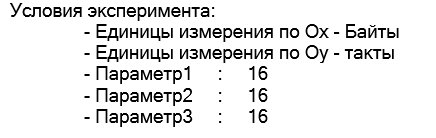
\includegraphics[scale=0.7]{tools/in_1.png}
	\caption{Условия эксперимента 1}
\end{figure}

\subsection{Результат эксперимента}
\begin{figure}[h]
	\centering
	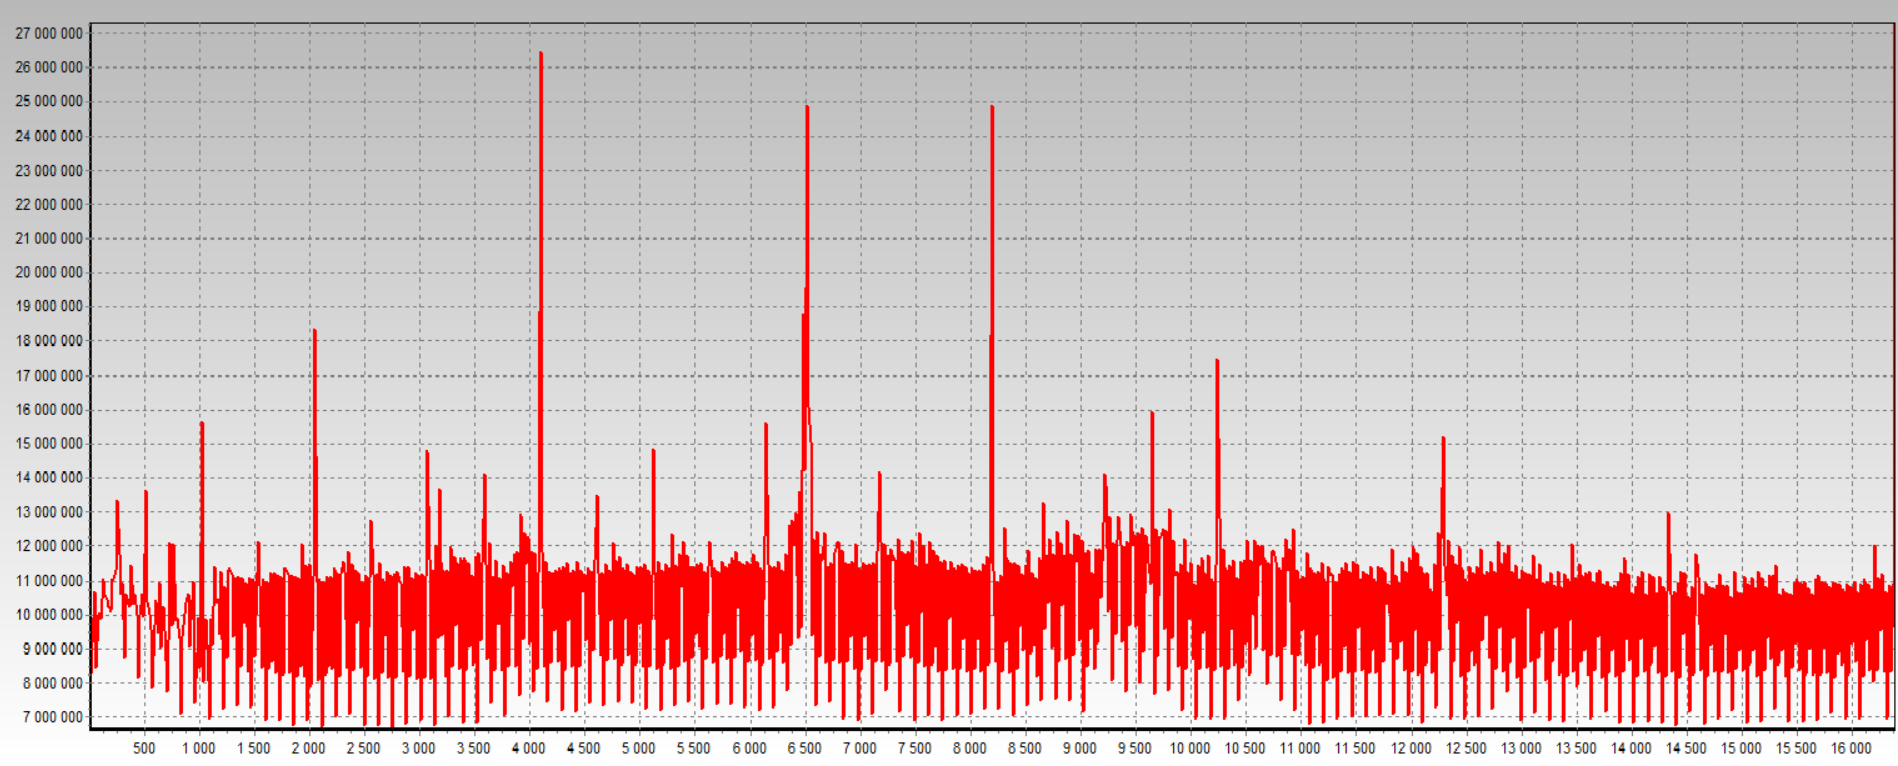
\includegraphics[scale=0.4]{tools/exp_1.png}
	\caption{Результат эксперимента 1}
\end{figure}

\subsection{Вывод}
Исходя из графика, минимальный шаг, при котором происходит постоянное обращение к одному и тому же банку T1 = 128; 
объем данных, являющийся минимальной порцией обмена кэш-памяти верхнего уровня с оперативной памятью П = 8;
количество банков памяти Б = 16; шаг чтения являющийся наихудшим при обращении к динамической памяти Т2 = 4096.

\clearpage\section{Эксперимент 2. Сравнение эффективности ссылочных и векторных структур}
\subsection{Условия эксперимента}
\begin{figure}[h]
	\centering
	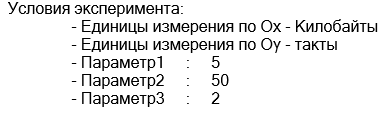
\includegraphics[scale=0.7]{tools/in_2.png}
	\caption{Условия эксперимента 2}
\end{figure}

\subsection{Результат эксперимента}
\begin{figure}[h]
	\centering
	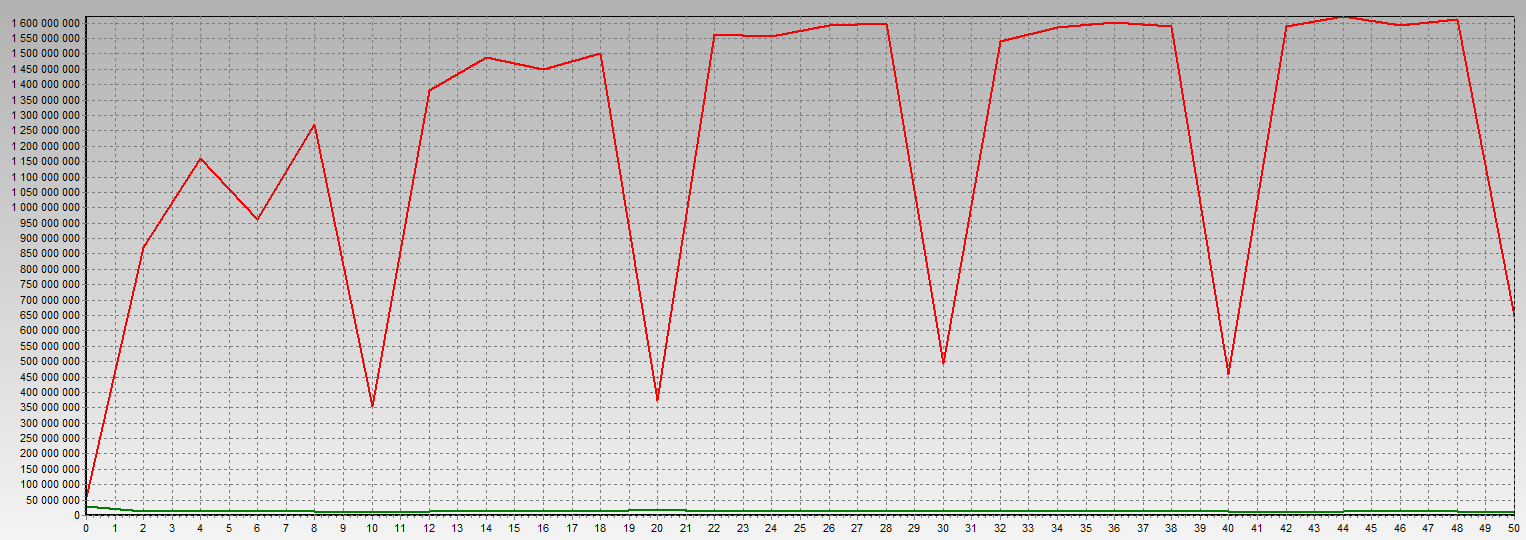
\includegraphics[scale=0.5]{tools/exp_2.png}
	\caption{Результат эксперимента 2}
\end{figure}

\subsection{Вывод}
Красный график показывает время или количество тактов работы алгоритма, использующего список. Зеленый график 
показывает время или количество тактов работы алгоритма, использующего массив. Очевидно, массив быстрее.

\clearpage\section{Эксперимент 3. Исследование эффективности программной предвыборки}
\subsection{Условия эксперимента}
\begin{figure}[h]
	\centering
	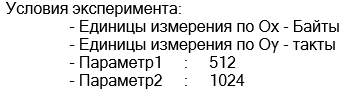
\includegraphics[scale=0.7]{tools/in_3.png}
	\caption{Условия эксперимента 3}
\end{figure}

\subsection{Результат эксперимента}
\begin{figure}[h]
	\centering
	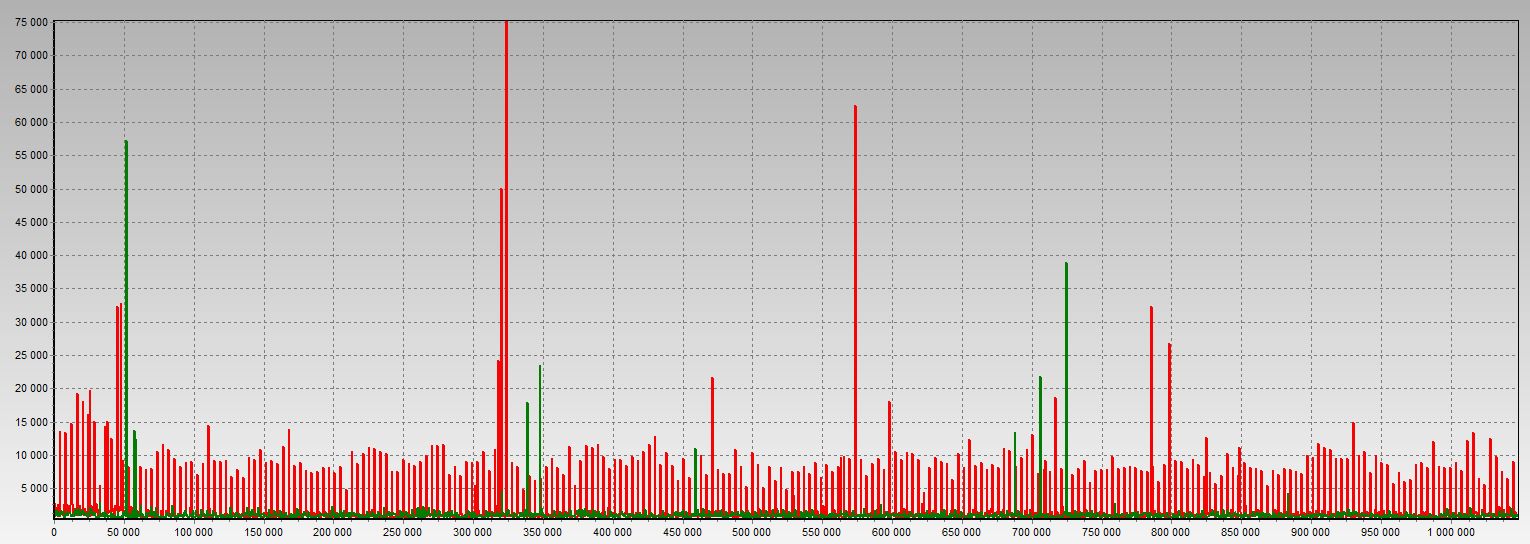
\includegraphics[scale=0.5]{tools/exp_3.png}
	\caption{Результат эксперимента 3}
\end{figure}

\subsection{Вывод}
Красный график показывает время или количество тактов работы алгоритма без предвыборки. Зеленый график показывает 
время или количество тактов работы алгоритма с использованием предвыборки. Алгоритм с использованием предвыборки 
работает быстрее.

\clearpage\section{Эксперимент 4. Исследование способов эффективного чтения оперативной памяти}
\subsection{Условия эксперимента}
\begin{figure}[h]
	\centering
	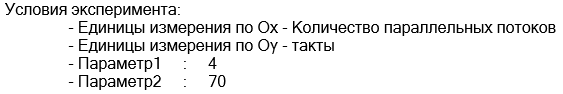
\includegraphics[scale=0.7]{tools/in_4.png}
	\caption{Условия эксперимента 4}
\end{figure}

\subsection{Результат эксперимента}
\begin{figure}[h]
	\centering
	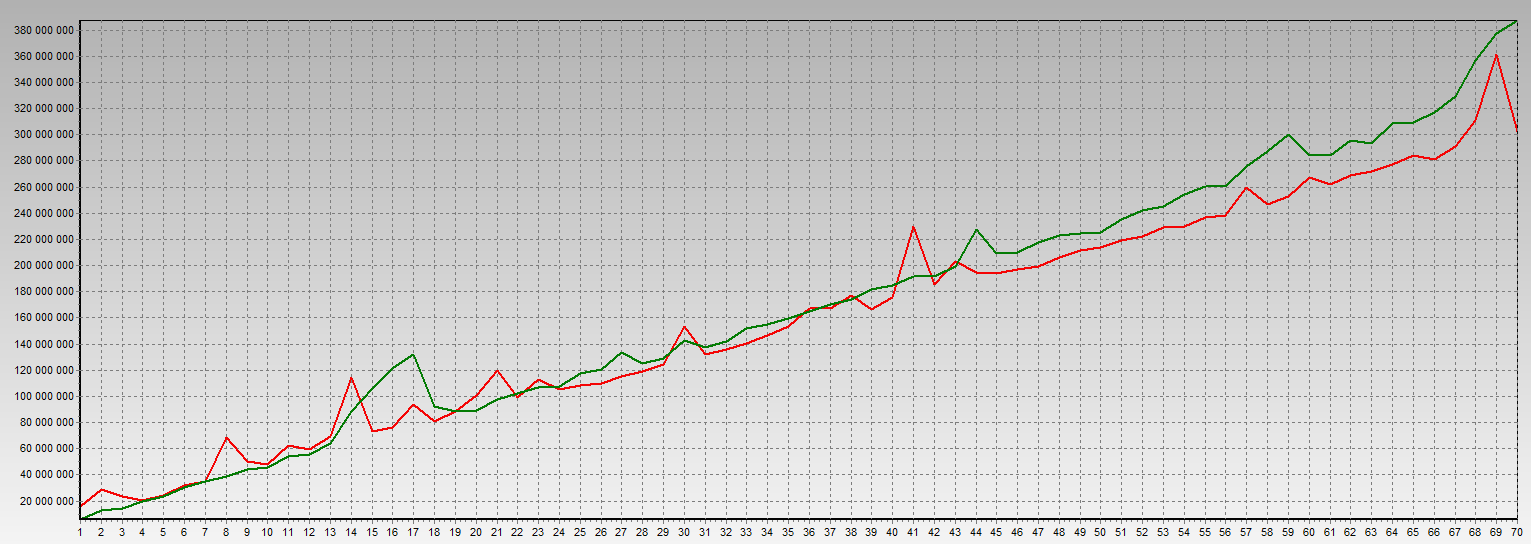
\includegraphics[scale=0.5]{tools/exp_4.png}
	\caption{Результат эксперимента 4}
\end{figure}

\subsection{Вывод}
Красный график показывает время или количество тактов работы алгоритма, использующего неоптимизированную  структуру. 
Зеленый график показывает время (или количество тактов) работы алгоритма с использованием оптимизированной структуры.
Алгоритм, использующий неоптимизированную структуру, быстрее.

\clearpage\section{Эксперимент 5. Исследование конфликтов в кэш-памяти}
\subsection{Условия эксперимента}
\begin{figure}[h]
	\centering
	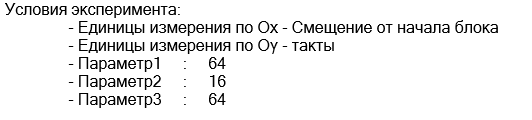
\includegraphics[scale=0.7]{tools/in_5.png}
	\caption{Условия эксперимента 5}
\end{figure}

\subsection{Результат эксперимента}
\begin{figure}[h]
	\centering
	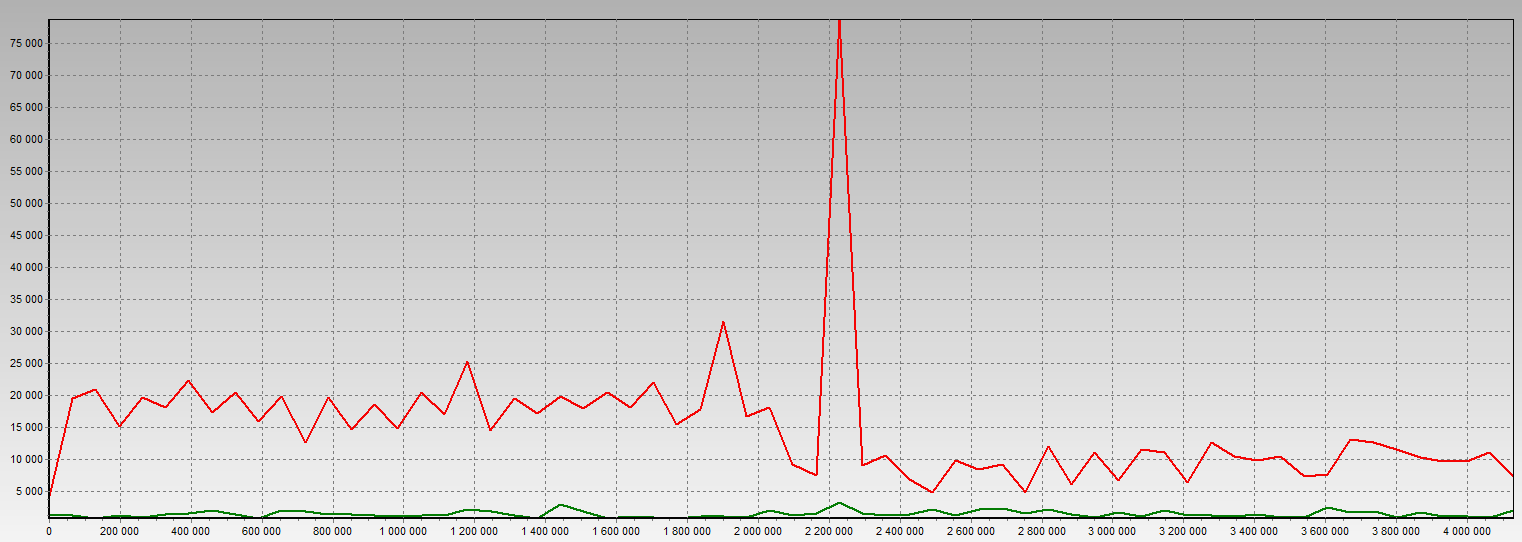
\includegraphics[scale=0.5]{tools/exp_5.png}
	\caption{Результат эксперимента 5}
\end{figure}

\subsection{Вывод}
Красный график показывает время или количество тактов работы процедуры, читающей данные с конфликтами в кэш-памяти. 
Зеленый график показывает время или количество тактов работы процедуры, не вызывающей конфликтов в кэш-памяти.
Процедура, не вызывающая конфликтов в кэш-памяти, быстрее.

\clearpage\section{Эксперимент 6. Сравнение алгоритмов сортировки}
\subsection{Условия эксперимента}
\begin{figure}[h]
	\centering
	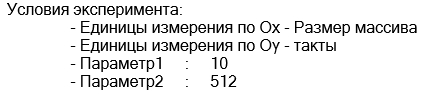
\includegraphics[scale=0.7]{tools/in_6.png}
	\caption{Условия эксперимента 6}
\end{figure}

\subsection{Результат эксперимента}
\begin{figure}[h]
	\centering
	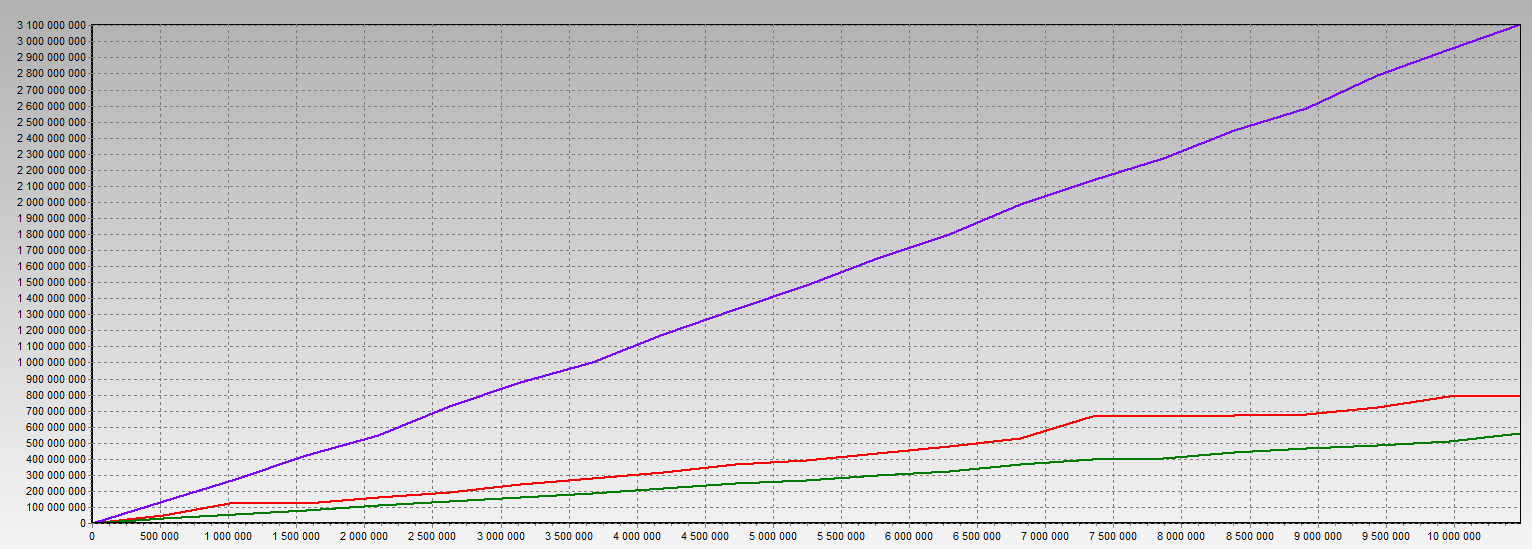
\includegraphics[scale=0.5]{tools/exp_6.png}
	\caption{Результат эксперимента 6}
\end{figure}

\subsection{Вывод}
Фиолетовый график показывает время или количество тактов работы алгоритма QuickSort. Красный график показывает время 
или количество тактов работы неоптимизированного алгоритма Radix-Counting. Зеленый график показывает время или 
количество тактов работы оптимизированного под 8-процессорную вычислительную систему алгоритма Radix-Counting. 
Самый быстрый алгоритм -- оптимизированный Radix-Counting, самый медленный -- QuickSort.

\clearpage\section{Ответы на контрольные вопросы}
\begin{enumerate}
	\item \textbf{Вопрос:} назовите причины расслоения оперативной памяти. \textbf{Ответ:} в связи с конструктивной 
неоднородностью оперативной памяти, обращение к последовательно расположенным данным требует различного времени.
	\item \textbf{Вопрос:} как в современных процессорах реализована аппаратная предвыборка. \textbf{Ответ:} с помощью 
кэша или  специальных таблиц адресов переходов BTB (Branch Target Buffer).
	\item \textbf{Вопрос:} какая информация храниться в TLB. \textbf{Ответ:} TLB хранит последние переводы виртуальной 
памяти в физическую память и может называться кэшем преобразования адресов.
	\item \textbf{Вопрос:} какой тип ассоциативной памяти используется в кэш-памяти второго уровня современных ЭВМ и 
почему. \textbf{Ответ:} 
	\item \textbf{Вопрос:} приведите пример программной предвыборки. \textbf{Ответ:} получение информации о 
преобразовании адресов из TLB буфера. 
\end{enumerate}

\end{document}